\begin{marginfigure}
\begin{tikzpicture}
\node [name-dest] (box){%
    \begin{minipage}{0.80\textwidth}
    \begin{itemize}
    \item Sam Page
    \item James 'Tetley' Hooper
    \end{itemize}
    \end{minipage}
};
\node[fancytitle, right=10pt] at (box.north west) {Beetle Juice};
\end{tikzpicture}
\end{marginfigure}

\section{Our Minds Were Full of Questions}

\paragraph{Sam 8.40am}

It had been my longest pushing trip to date, and my first time beyond Stuck in Paradise. Our pushing target had been \#, in which we had great fun squeezing ourselves through the twisty-turny tunnels. Once we had reached a point at which we felt we could progress no further through the ever narrowing passage, we surveyed our way back, adding a small number of metres to the survey. Tetley was keen to check out some of the newly discovered cave nearby – particularly Atlantis and its formations. Given our relative proximity to this area, I agreed to go along with this plan, although I think I was ready to return to camp already at this point.

\margininbox{Sam 5.40am}{Tet’s gone all philosophical...}

We ventured down to Atlantis, and without hanging about for too long, began the long trip back to camp. Our plan was slow-and-steady, with plenty of rest breaks. I was the first to arrive at Hawaii, and sat down to catch my breath and have a drink. Something caught my eye, movement in the rocks. I looked down and there was an animal beside me! It was a kind of small, furry rodent, black with a long fluffy tail. At this point, Tetley was clambering over the rocks to join me. I anxiously asked him “Look at this - What is it?!”, and when he noticed the animal, he gave a shriek. The animal then moved off and disappeared under some rocks and we did not see it again. This all happened within a short number of seconds. Our minds were full of questions. What was it? Where did it come from? How did it get to this bit of cave? How does this make us feel? 

\margininbox{Tetley 7.30pm}{Talking of Petzl, as a boy I read his tales of cave exploration, also the stories of Dent de Crolles, PSM, Gouffre Berger etc. Looking now at the survey of our 25km system (hopefully now 30km+ if Primadona/Monatip has now connected in) it really is amazing, truly amazing, that we’ve a tale and a cave of similar magnitude!
I’m feeling sleepy again so I’ll spare you my musing on love/relationships...}

Of course, our journey back to camp remained. Our discovery of the animal remained on our minds throughout. Assuming that it did not live in the cave (revolutionising science), it must have come from the surface. How then did it arrive at Hawaii, somewhere which to the best of our knowledge was deep underground and far removed from any of the cave entrances? Probably given the length of our pushing trip and tiredness, our minds roamed to stranger explanations, of aliens or hallucinations or magic. More often, we just laughed at the peculiarity of our experience. 

We had camp to ourselves, and I seemingly slept for 17 hours(!). We decided against a third day of pushing, instead to make our way back to the surface. The concoction of thoughts surrounding the creature we found was intensified by the time we spent underground without seeing another person. We were desperate to be able to tell everyone about what we had seen, and to see if they believed us or not. Given that we saw the animal for such a short period of time, and me the longest of the two of us, it was easy to question if we really had seen such a thing. For the sake of our sanity, we decided that we had. 




\name{Sam Page}

\section{The Minds in Question}

Just back from our trip and I am ever so slightly broken...
More Importantly, WE ARE NOT ALONE! Me and Tetley saw a fucking animal at Hawaii. It was some sort of mix between a rat and a squirrel, black with a long fluffy black tail. Something like this. \ref{fig:the_creature}
After I sat down I turned my head an it was just there. My first reaction was to ask Tetley “What is THAT?”; his first reaction was to scream as it moved and ran away. I probably watched it for around ten seconds before it disappeared. Where did it come from to end up at -800m!?! Does this mean there is an entrance somewhere around there. How could it get to where we were; it looked like it was moving well yet was spooked by us. We too were spooked by it. Surely it and more of it’s kind don’t live down here with us? First action when back on the surface is to find out if such a creature exists.
P.S. Creature Theories
\begin{citemize}
\item 1. Saber brought it down in a cage and released it
\item 2. It came from outside
\item 3. Tetley and Sam had a mad hallucinogenic trip
\item 4. An alien invasion of Sys Mig
\item 5. A creature to revolutionise all known biology - where does it get its light/food from???
\item 6. Magic
\end{citemize}

\begin{figure}[t!]
	\checkoddpage \ifoddpage \forcerectofloat \else \forceversofloat \fi
	\centering
	\frame{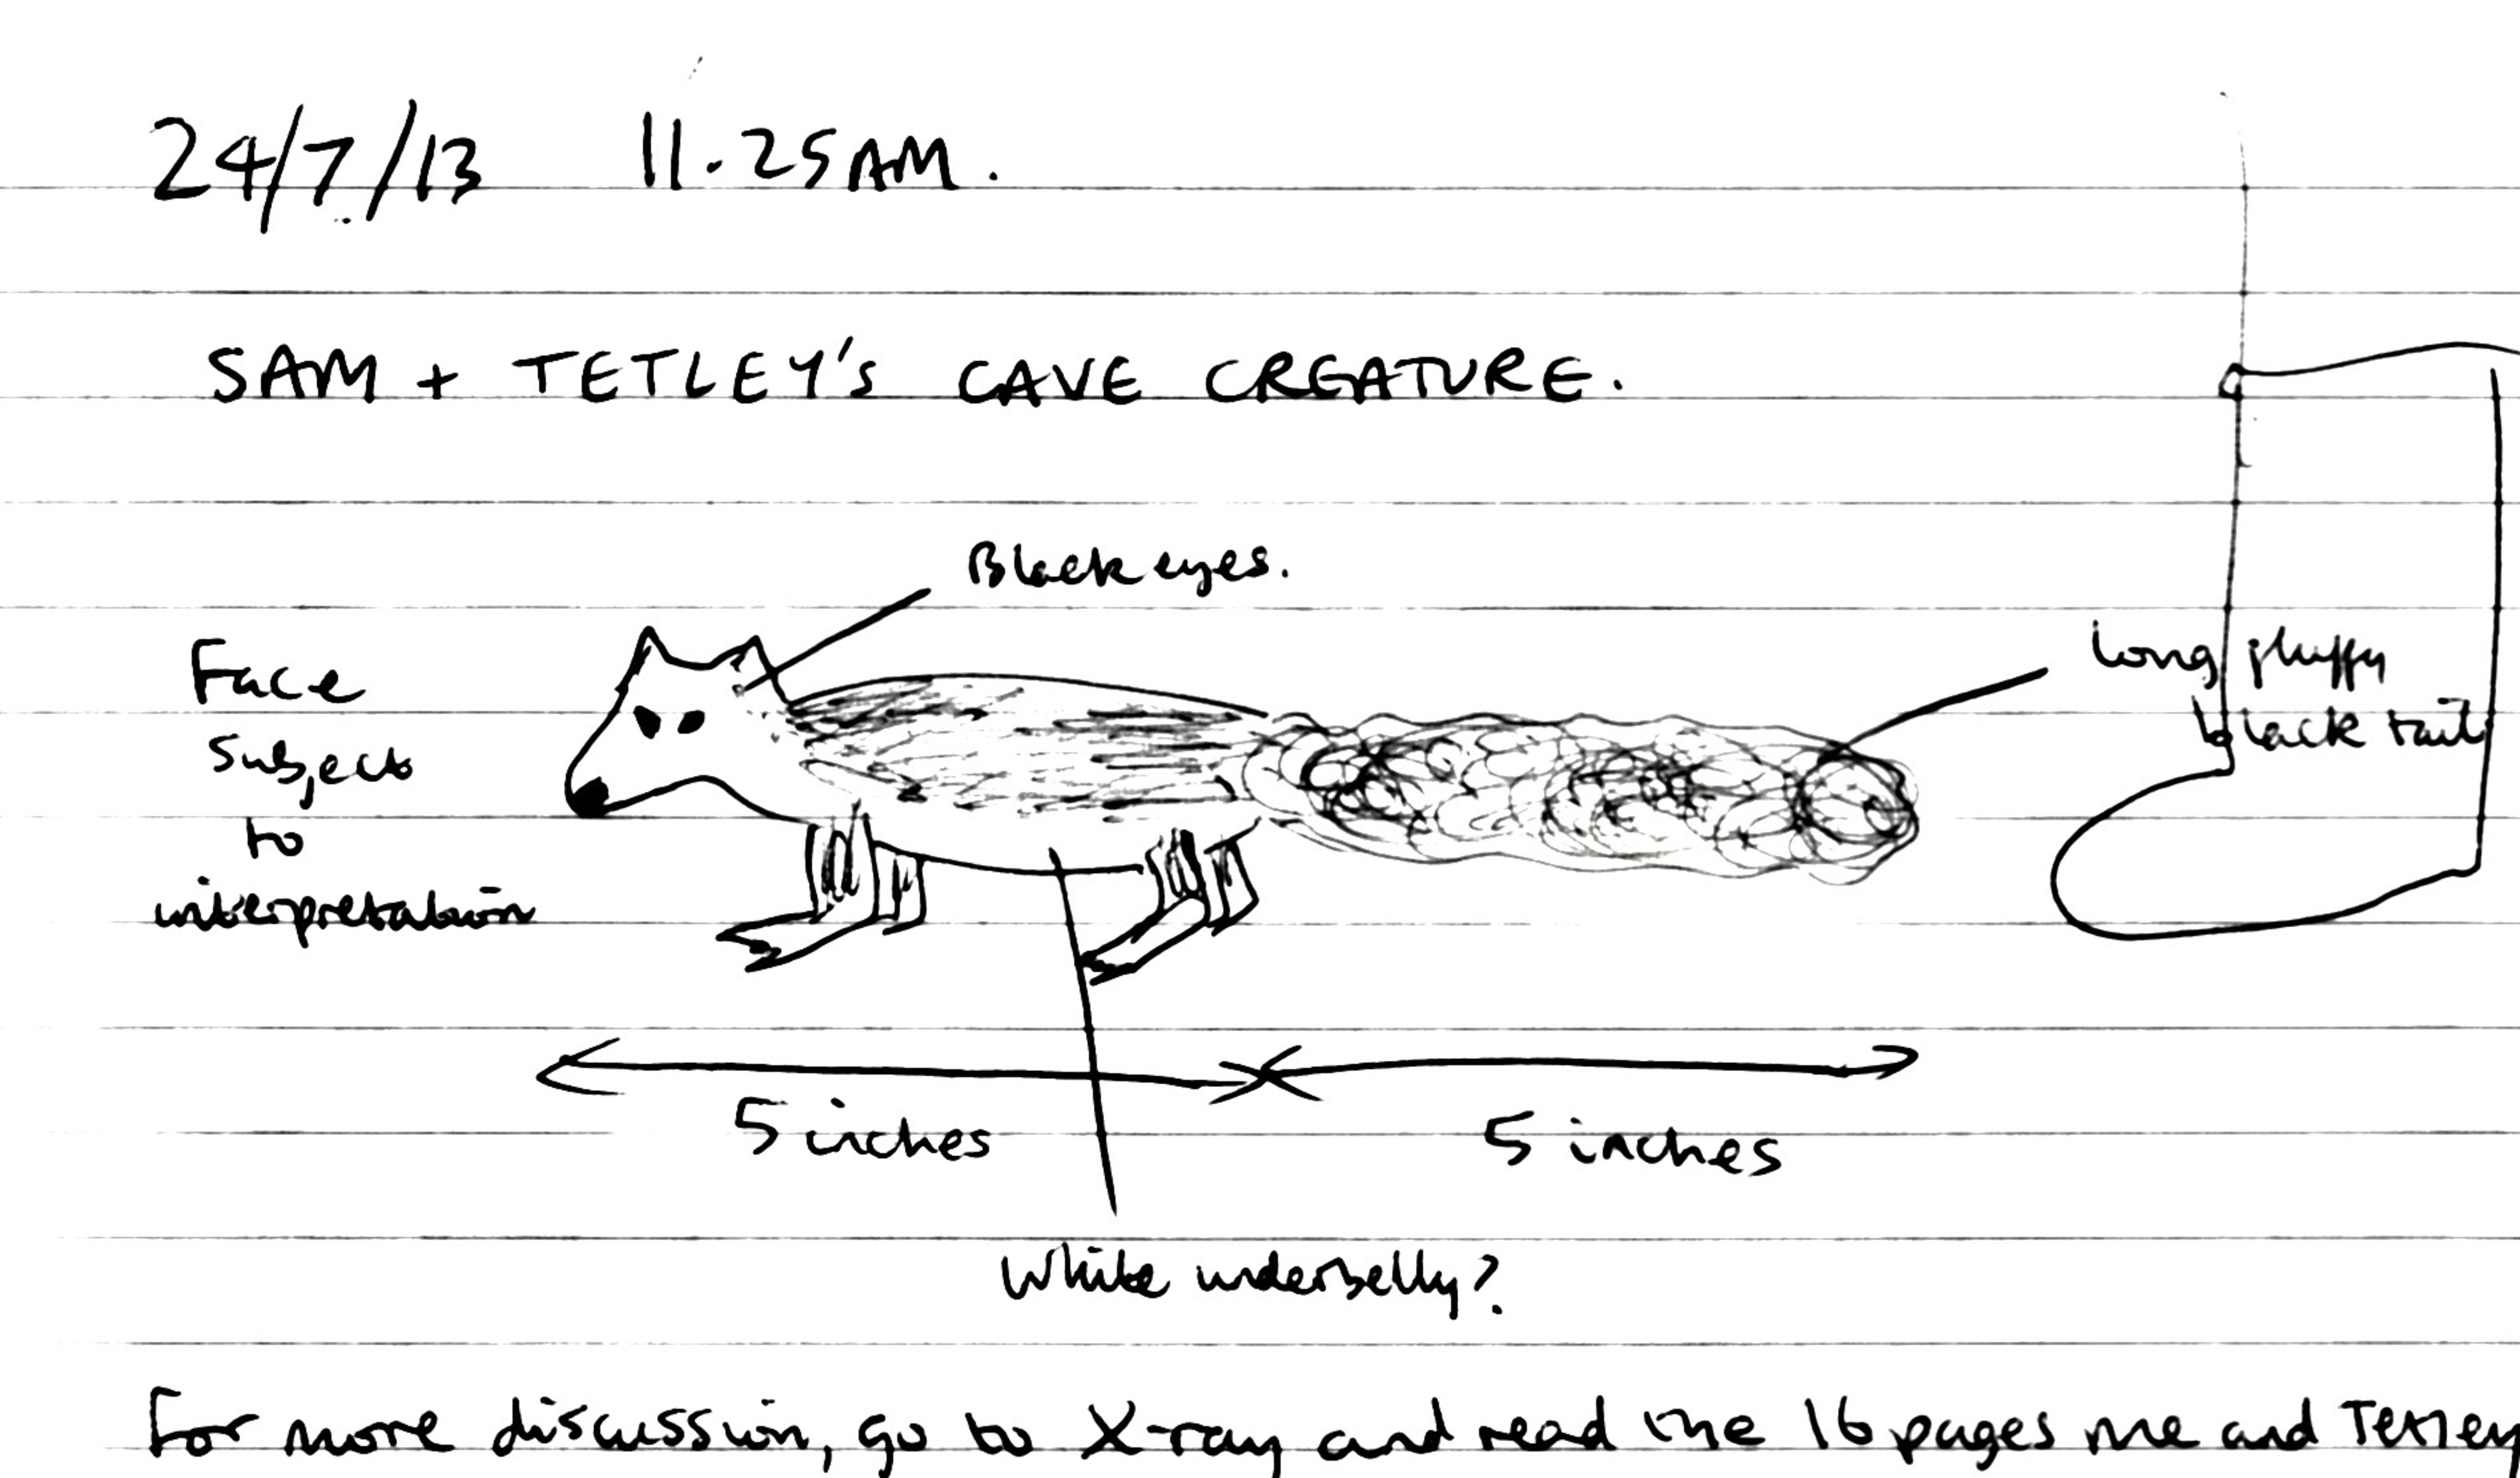
\includegraphics[width=\textwidth]{images/2013/tetley-sam-2013/creature.pdf}}
	\caption{The creature spotted by Sam and Tetley, drawn in the 2013 scanned logbook --- scanned, from Sam Page}
	\label{the_creature}
\end{figure}


\paragraph{Tetley 7.30pm}

So our trip yesterday... a smooth journey down to Hawaii. Stuck in Paradise is much much better than when I first went down but still somewhat muddy and loose. Sam’s first trip to this part of the cave. We had vitaminski tea and hot fish sandwiches. Went to push HASH, added 25m (Sam described this earlier). The leas isn’t great but it is still draughting and going. We then went to see the nice stal at Atlantis, very pretty! Back to Hawaii for tea...Sam was ahead of me and as I neared Hawaii said, with I detected a slight anxious tone in his voice, “Tetley, tetley look at this”. I was thinking maybe he was watching a spider or something...I approached and there to my surprise (to put it mildly) was a rat type creature. It moved! I screamed!

What! Why? How? We had some ginger cake (leaving some for the creature), also had some vitaminski tea. Dumbfounded we headed back to camp...

\paragraph{Sam 5.20am}
Been at x-ray for an awfully -wrong word- brilliantly long time now. I don't expect I would have been able to sleep for 17 hours on the surface. 3 days of just Tetley and I (plus our mysterious creature still preoccupying our thoughts) - where have all the cavers gone? Presumably the connection with Monatip/B12/the Bivvy have proven too distracting. Plan is to head out at some point today, as long as we are out for sunset. Before that, food, more sleep, Rum Doodle, Blackadder....good times.

\paragraph{Tetley 6.10am}
6 billion people on the planet and no-one can have had a weekend like the one Sam and I had! Now eating cheesy, soupy, fishy, smash (classic! with - and highly recommended - fresh onion. More Rum Doodle, Black Adder, sleep now...

\begin{figure*}[b!]
\begin{tikzpicture}
\node [name-dest] (box){%
    \begin{minipage}{0.95\textwidth}
    \begin{multicols}{2}
    \paragraph{General characters of the dormouse}  The edible dormouse \emph{Glis Glis} is the largest of its genus and has the appearance of a squirrel. Both sexes are roughly the same size with a body of length averaging 15.3cm, and tail measuring 12.5cm \citep{kryvstufek2001compartmentalisation}. Its pelage consist of a soft underfur, mixed with coarser, longer guard hairs along the back. The fur ranges from grey-brown to smoke-grey and is darkest along the spine. The underparts are white to pale buff, and the transition is clearly defined. The tail has the same colour as the back, albeit darker.
    \paragraph{distribution} \emph{Glis Glis} is widespread in the deciduous western, central and southeastern Europe except near the Atlantic and North sea coasts.  It is found from sea level to the upper margins of deciduous and mixed forests, at elevations of up to 2000m in the Pyrenees \citep{spitzenberger2001saugetierfauna}. The edible dormouse, very widespread in Slovenia \citep{kryvstufek1991sesalci} is a nocturnal arboreal rodent which uses tree hollows, as well as burrows to breed. Their occurrence in caves has been known about for centuries \citep{von1994slava}, as Slovene hunters caught the fat dormice outside \emph{pol\v{s}ine}, very small entrances (5 -10cm diameter) to larger cave systems, where the rodents are found to nest and hibernate \citep{scaravelli1995myoxus}.
    \paragraph{occurrence in caves} Dormice commonly occur in caves of the Slovene Dinaric karst, a mountainous area covered with a mixture of beech (\emph{Fagus Sylvatica}) and fir (\emph{Abieti-fagetum dinaricum}) forests \citep{polak1997}.
    \end{multicols}{2}
    \end{minipage}};
\node[fancytitle, right=10pt] at (box.north west) {More about the edible dormouse \emph{Glis Glis}};
\end{tikzpicture}
\end{figure*}

\begin{pagefigure}
	\centering
	\begin{subfigure}{\linewidth}
		\frame{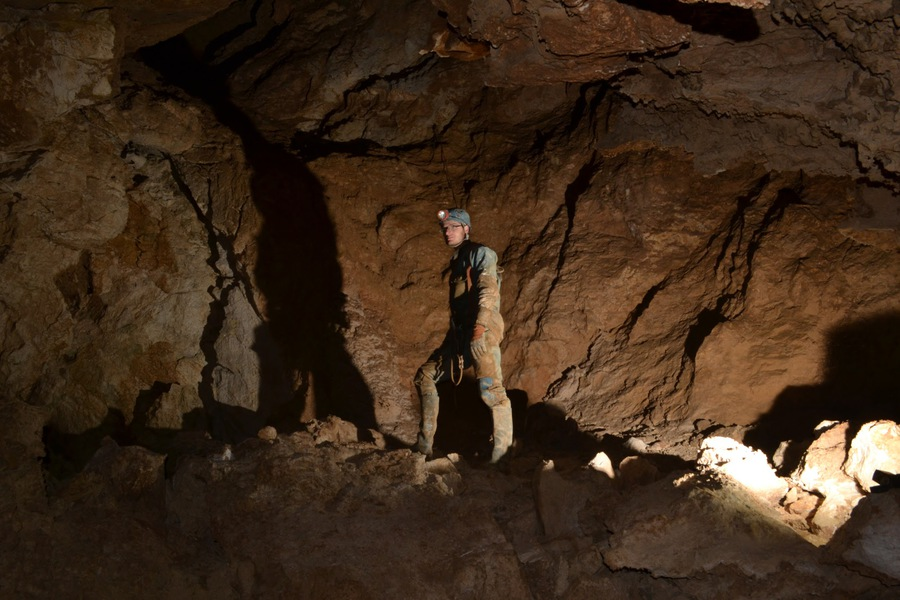
\includegraphics[width=\linewidth]{images/2013/tetley-sam-2013/rhys_hawaii.jpg}}
		\caption{}
		\label{hawaii}
	\end{subfigure}
	\vspace{5pt}
	\begin{subfigure}{\linewidth}
		\frame{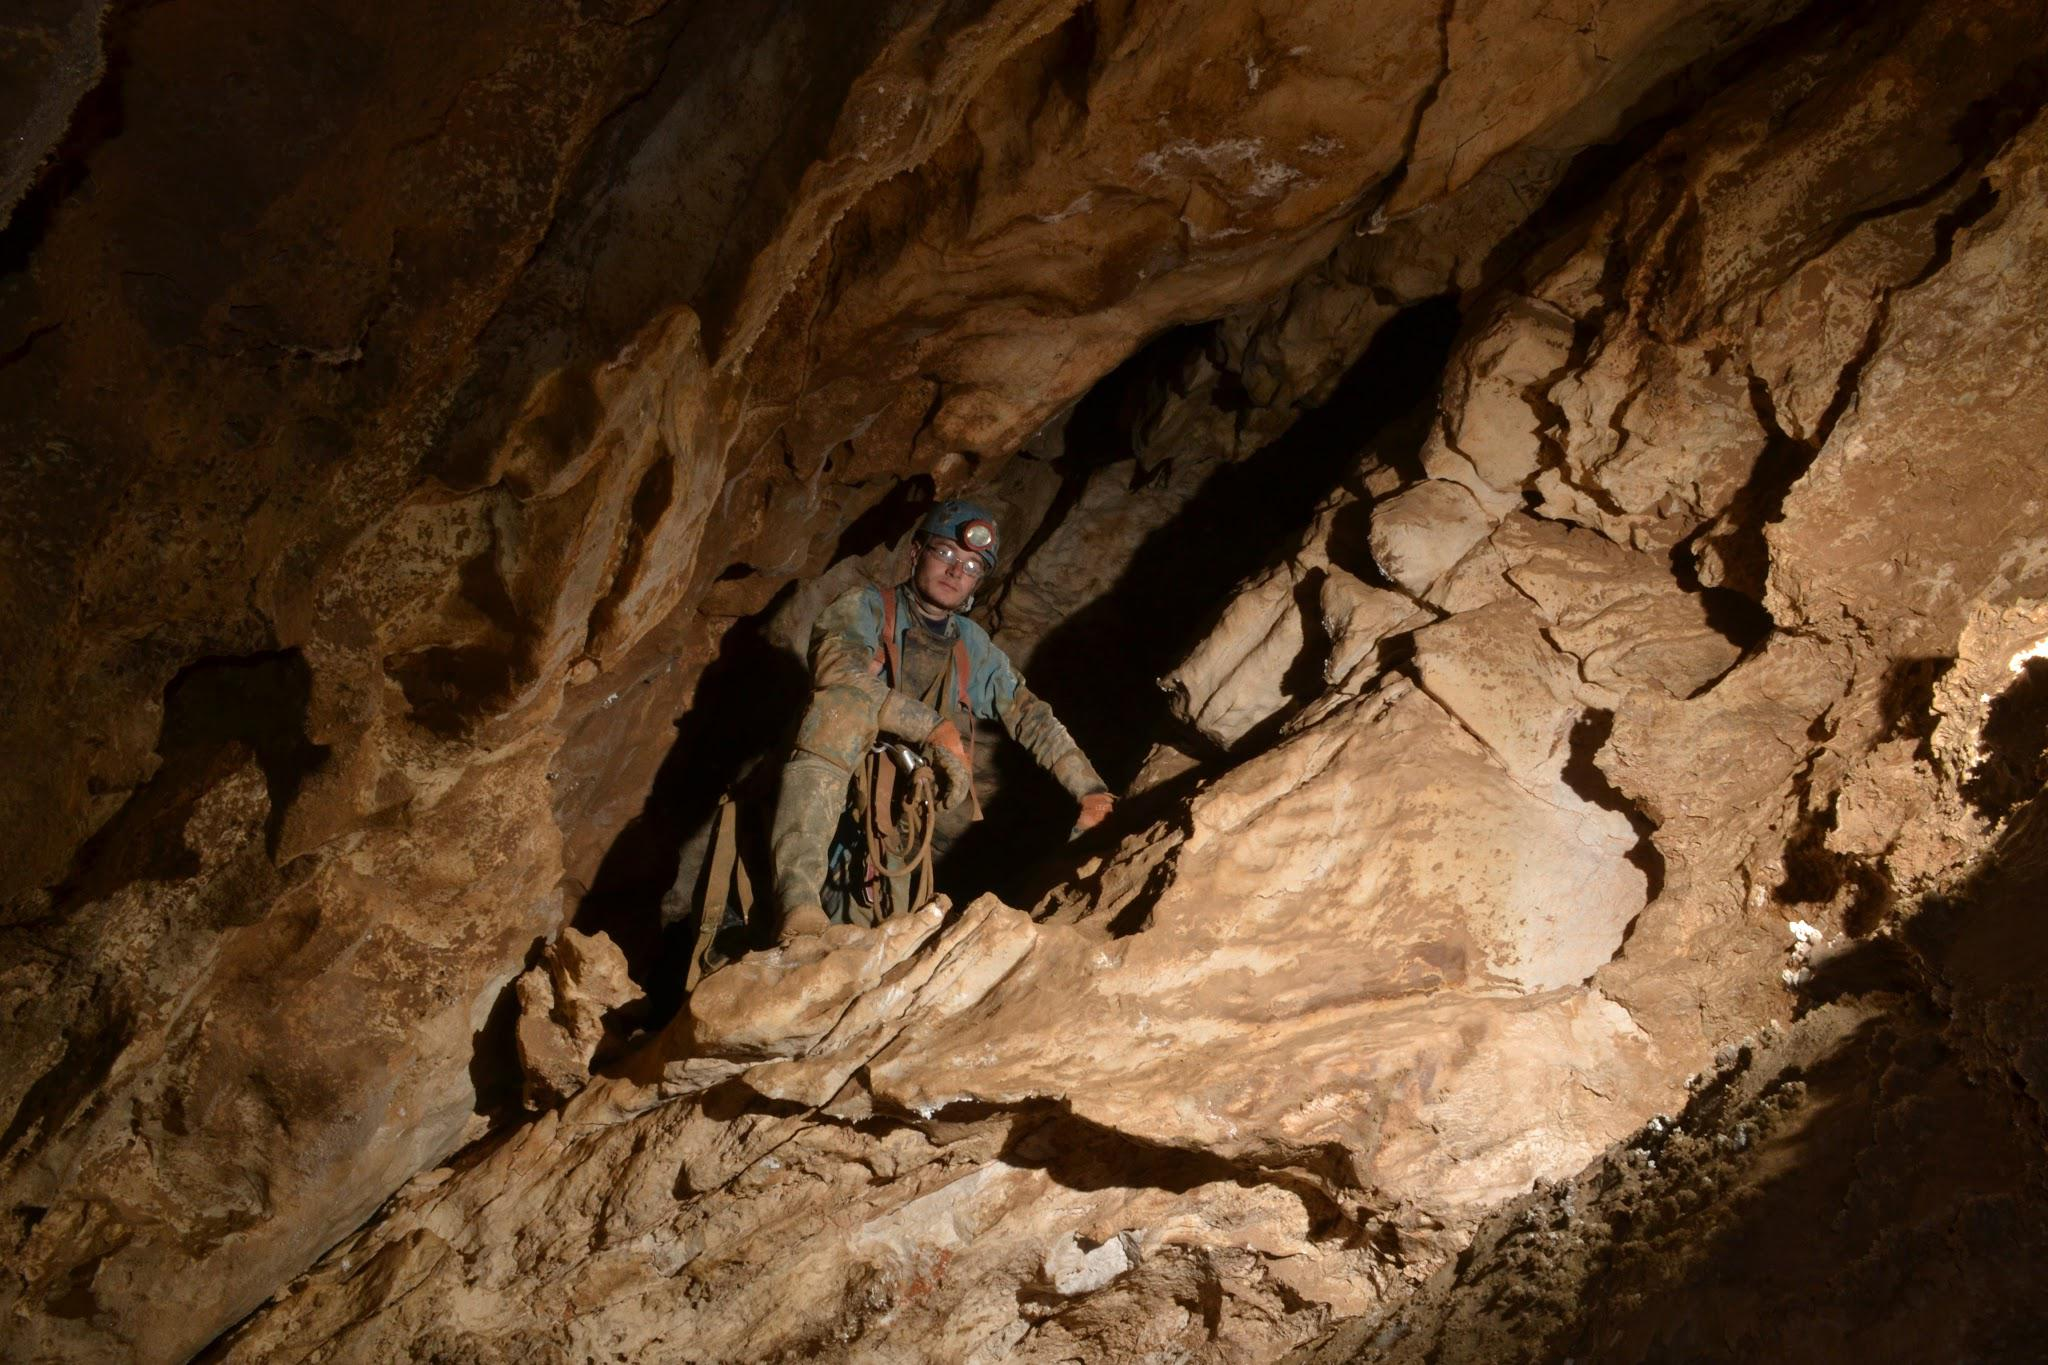
\includegraphics[width=\linewidth]{images/2013/tetley-sam-2013/rhys_lost_miles.jpg}}
		\caption{}
		\label{lostmiles}
	\end{subfigure}
	\caption{\emph{(a)} \protect\passage{Hawaii} junction, at the bottom of th extremely muddy \protect\passage{Stuck in Paradise} pitch \emph{(b)} \protect\passage{Lost Miles} passage --- Rhys Tyers}
	\label{}
\end{pagefigure}